\documentclass[color=usenames,dvipsnames]{beamer}\usepackage[]{graphicx}\usepackage[]{color}
% maxwidth is the original width if it is less than linewidth
% otherwise use linewidth (to make sure the graphics do not exceed the margin)
\makeatletter
\def\maxwidth{ %
  \ifdim\Gin@nat@width>\linewidth
    \linewidth
  \else
    \Gin@nat@width
  \fi
}
\makeatother

\definecolor{fgcolor}{rgb}{0.345, 0.345, 0.345}
\newcommand{\hlnum}[1]{\textcolor[rgb]{0.686,0.059,0.569}{#1}}%
\newcommand{\hlstr}[1]{\textcolor[rgb]{0.192,0.494,0.8}{#1}}%
\newcommand{\hlcom}[1]{\textcolor[rgb]{0.678,0.584,0.686}{\textit{#1}}}%
\newcommand{\hlopt}[1]{\textcolor[rgb]{0,0,0}{#1}}%
\newcommand{\hlstd}[1]{\textcolor[rgb]{0.345,0.345,0.345}{#1}}%
\newcommand{\hlkwa}[1]{\textcolor[rgb]{0.161,0.373,0.58}{\textbf{#1}}}%
\newcommand{\hlkwb}[1]{\textcolor[rgb]{0.69,0.353,0.396}{#1}}%
\newcommand{\hlkwc}[1]{\textcolor[rgb]{0.333,0.667,0.333}{#1}}%
\newcommand{\hlkwd}[1]{\textcolor[rgb]{0.737,0.353,0.396}{\textbf{#1}}}%
\let\hlipl\hlkwb

\usepackage{framed}
\makeatletter
\newenvironment{kframe}{%
 \def\at@end@of@kframe{}%
 \ifinner\ifhmode%
  \def\at@end@of@kframe{\end{minipage}}%
  \begin{minipage}{\columnwidth}%
 \fi\fi%
 \def\FrameCommand##1{\hskip\@totalleftmargin \hskip-\fboxsep
 \colorbox{shadecolor}{##1}\hskip-\fboxsep
     % There is no \\@totalrightmargin, so:
     \hskip-\linewidth \hskip-\@totalleftmargin \hskip\columnwidth}%
 \MakeFramed {\advance\hsize-\width
   \@totalleftmargin\z@ \linewidth\hsize
   \@setminipage}}%
 {\par\unskip\endMakeFramed%
 \at@end@of@kframe}
\makeatother

\definecolor{shadecolor}{rgb}{.97, .97, .97}
\definecolor{messagecolor}{rgb}{0, 0, 0}
\definecolor{warningcolor}{rgb}{1, 0, 1}
\definecolor{errorcolor}{rgb}{1, 0, 0}
\newenvironment{knitrout}{}{} % an empty environment to be redefined in TeX

\usepackage{alltt}
%\documentclass[color=usenames,dvipsnames,handout]{beamer}

%\usepackage[roman]{../pres1}
\usepackage[sans]{../pres1}
\usepackage{changepage}
\usepackage{array}
\usepackage{soul}




\IfFileExists{upquote.sty}{\usepackage{upquote}}{}
\begin{document}

%\fontfamily{lmodern}

\begin{frame}[plain]
  \begin{center}
    {\huge Estimating survival using telemetry \\ 
      \only<1>{{or age distribution data \\}}
      \only<2>{\st{or age distribution} data \\}}
%    \vspace{0.5cm}
%    { \Large April 17, 2019} \\
    {\color{blue} \rule{\textwidth}{0.1pt}}
    \vfill
    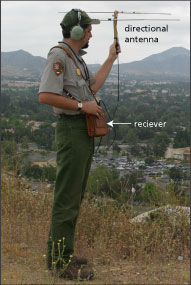
\includegraphics[height=4.5cm,keepaspectratio]{figs/radiotelemetry} %\hfill
    \hspace{0.5cm}
      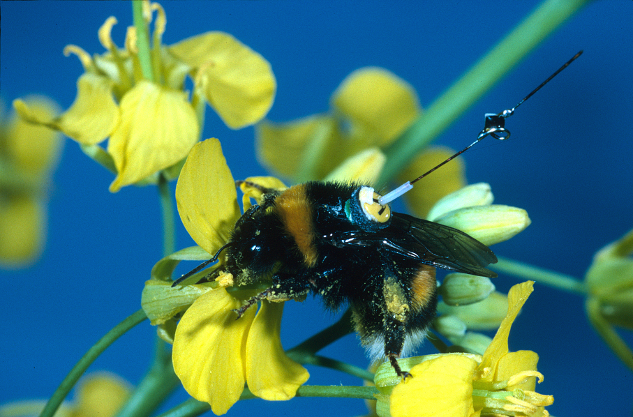
\includegraphics[height=4.5cm,keepaspectratio]{figs/bbee}
  \end{center}
\end{frame}




\section{Introduction}


\begin{frame}
  \frametitle{Introduction}
%  \huge \centering
%  Why not estimate yearly abundance and call it a day? \\
  \Large %\large
  {%\bf
    Options}
  \begin{enumerate}[\bf (1)]
    \large
    \item[]
    \item Telemetry
      \begin{itemize}
        \large
        \item Binomial model
        \item Kaplan-Meier model
      \end{itemize}
    \item[]
    \item<2-> Age distribution data
      \begin{itemize}
        \item Often used but rarely valid
      \end{itemize}
    \item[]
    \item<3-> Capture-mark-recapture
      \begin{itemize}
        \item Covered in the previous lecture
      \end{itemize}
  \end{enumerate}
\end{frame}




\section{Telemetry}



% \begin{frame}
%   \frametitle{Telmetry}
%   \begin{center}
%     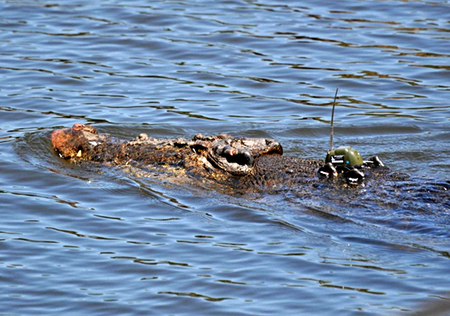
\includegraphics[width=0.9\textwidth]{figs/saltie}
%   \end{center}
% \end{frame}



\begin{frame}
  \frametitle{Telemetry}
  \begin{columns}
    \begin{column}{0.5\textwidth}
      {\large%\bf
        Pros}
      \begin{itemize}
        \item Fate is often known
        \item Analysis can be straight-forward
        \item Much additional information can be obtained
      \end{itemize}
      \uncover<2->{\large %\bf
        {Cons}}
      \begin{itemize}[<2->]
        \item Batteries don't last as long as bands
        \item When fate is unknown, analysis can be hard
        \item Transmitters may influence vital rates and behavior
      \end{itemize}
    \end{column}
    \begin{column}{0.5\textwidth}
      \includegraphics<1->[width=\textwidth]{figs/saltie} \\
      \vfill
      \uncover<2->{\includegraphics[width=\textwidth]{figs/Banded_Penguin}}
    \end{column}
  \end{columns}
\end{frame}



% \begin{frame}
%   \frametitle{Design}
%   Sample must be representative
% \end{frame}



\begin{frame}
  \frametitle{Binomial model}
  \large
  {%\bf
    Design}
  \begin{itemize}%[<+->]
    \normalsize
    \item<1-> $n$ animals are randomly sampled %from population of size $N$
    \item<2-> The fates of all $n$ are known at end of the study period
    \item<3-> $x$ of the $n$ animals survive
    \item<4-> The estimate of survival over the time interval is:
  \end{itemize}
  \pause
%  \LARGE
  \Large
  \vspace{0.5cm}
  \uncover<4->{
  \[
    \hat{S} = \frac{x}{n}
  \]}
\end{frame}



\begin{frame}
  \frametitle{Binomial model}
  \large
  {%\bf
    Assumptions}
  \begin{enumerate}[(1)]%[\bf (1)] %[<+- | visible@+->][\bf \color{PineGreen} (1)]
    \normalsize
    \item<1-> Fates are independent
    \item<1-> Fates are known
    \item<1-> All individuals are exposed to mortality during the same time interval
  \end{enumerate}
%  \pause
  \vspace{0.5cm}
%  \bf
  \uncover<2->{\centering When \alert{censoring} occurs, assumptions
    (2) and (3) are violated \par}
  \vspace{0.5cm}
  \uncover<3>{Censoring occurs when the time of mortality is not
    directly observed}
\end{frame}





\begin{frame}
  \frametitle{Censoring}
  {\large %\bf
    Right censoring} 
  \begin{itemize}
    \normalsize
    \item Occurs when animals leave the sample before they die.
    \item Examples
    \begin{itemize}
      \item Battery failure
      \item Emigration
    \end{itemize}
%    \item If right-censored animals are incorrectly thought to be dead,
%      survival estimates will be biased low
  \end{itemize}
  \pause
  \vfill
  {\large %\bf
    Left censoring and interval censoring are rarely a concern}
  % \begin{itemize}
  %   \normalsize
  %   \item Occurs when mortality is known to have occurred before some
  %     point in time
  %   \item Rarely an issue in telemetry studies
%    \item Also known as ``staggered entry''
%    \item If left-censored animals are incorrectly thought to enter
%      the study at $t=1$, survival estimates will be biased high
  % \end{itemize}
  \pause
  \vfill
  {\centering If censoring occurs, 
    the Kaplan-Meier estimator is more appropriate than the binomial model. \\}
\end{frame}



\begin{frame}
  \frametitle{Censoring}
%  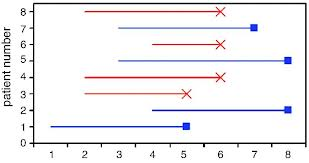
\includegraphics[width=0.9\textwidth]{figs/censor}
  \centering
  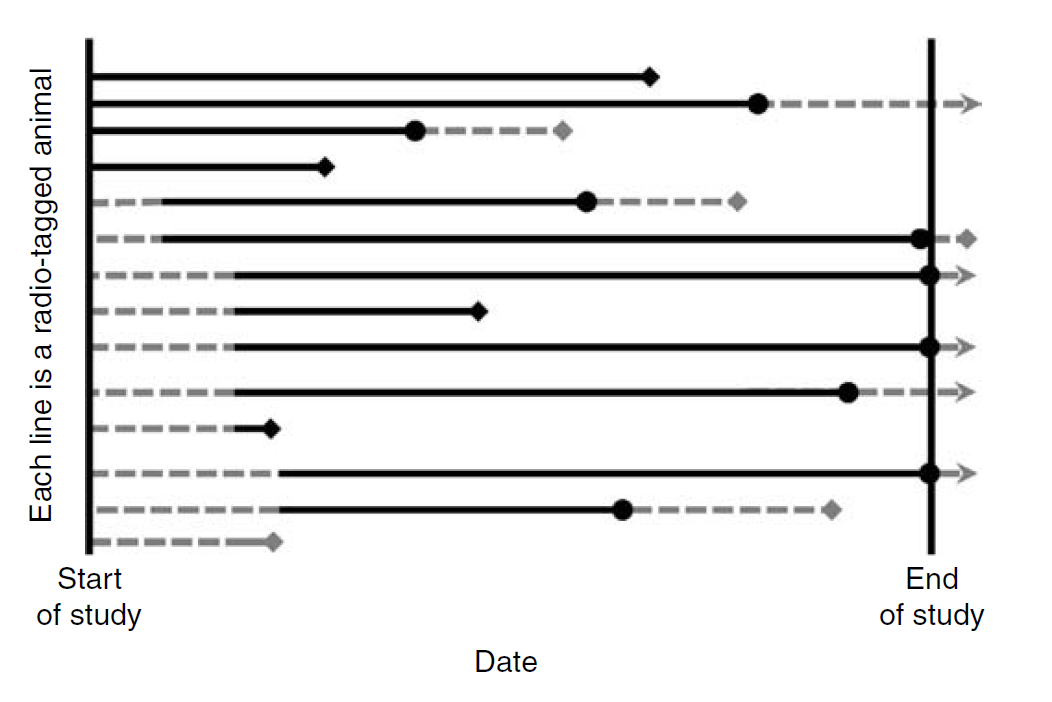
\includegraphics[width=0.9\textwidth]{figs/censoring} \\
  Diamonds indicate mortality. Circles indicate censoring. \\
  Black lines show the observation period. \\ %Gray lines are unobserved
  %time periods. 
\end{frame}


\begin{frame}
  \frametitle{Kaplan-Meier}
  \LARGE
  \[
    \hat{S}_t = \prod_{j: t_i \le t}\left(\frac{r_j - d_j}{r_j}\right)
  \]
  \large
  $S_t$ -- probability of surviving to time $t$ \\
  $r_j$ -- number of individuals ``at risk'' prior to time $t$ \\
  $d_j$ -- number of mortalities prior to time $t$
\end{frame}



\begin{frame}
  \frametitle{Kaplan-Meier}
  \begin{center}
%    \Large
%    Survivorship curve \\
%    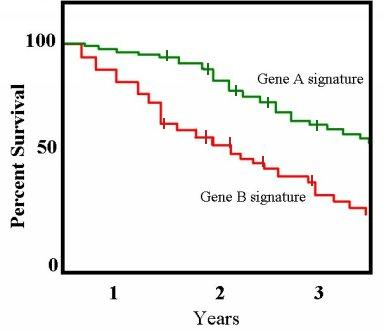
\includegraphics[width=0.6\textwidth]{figs/survivorship}
    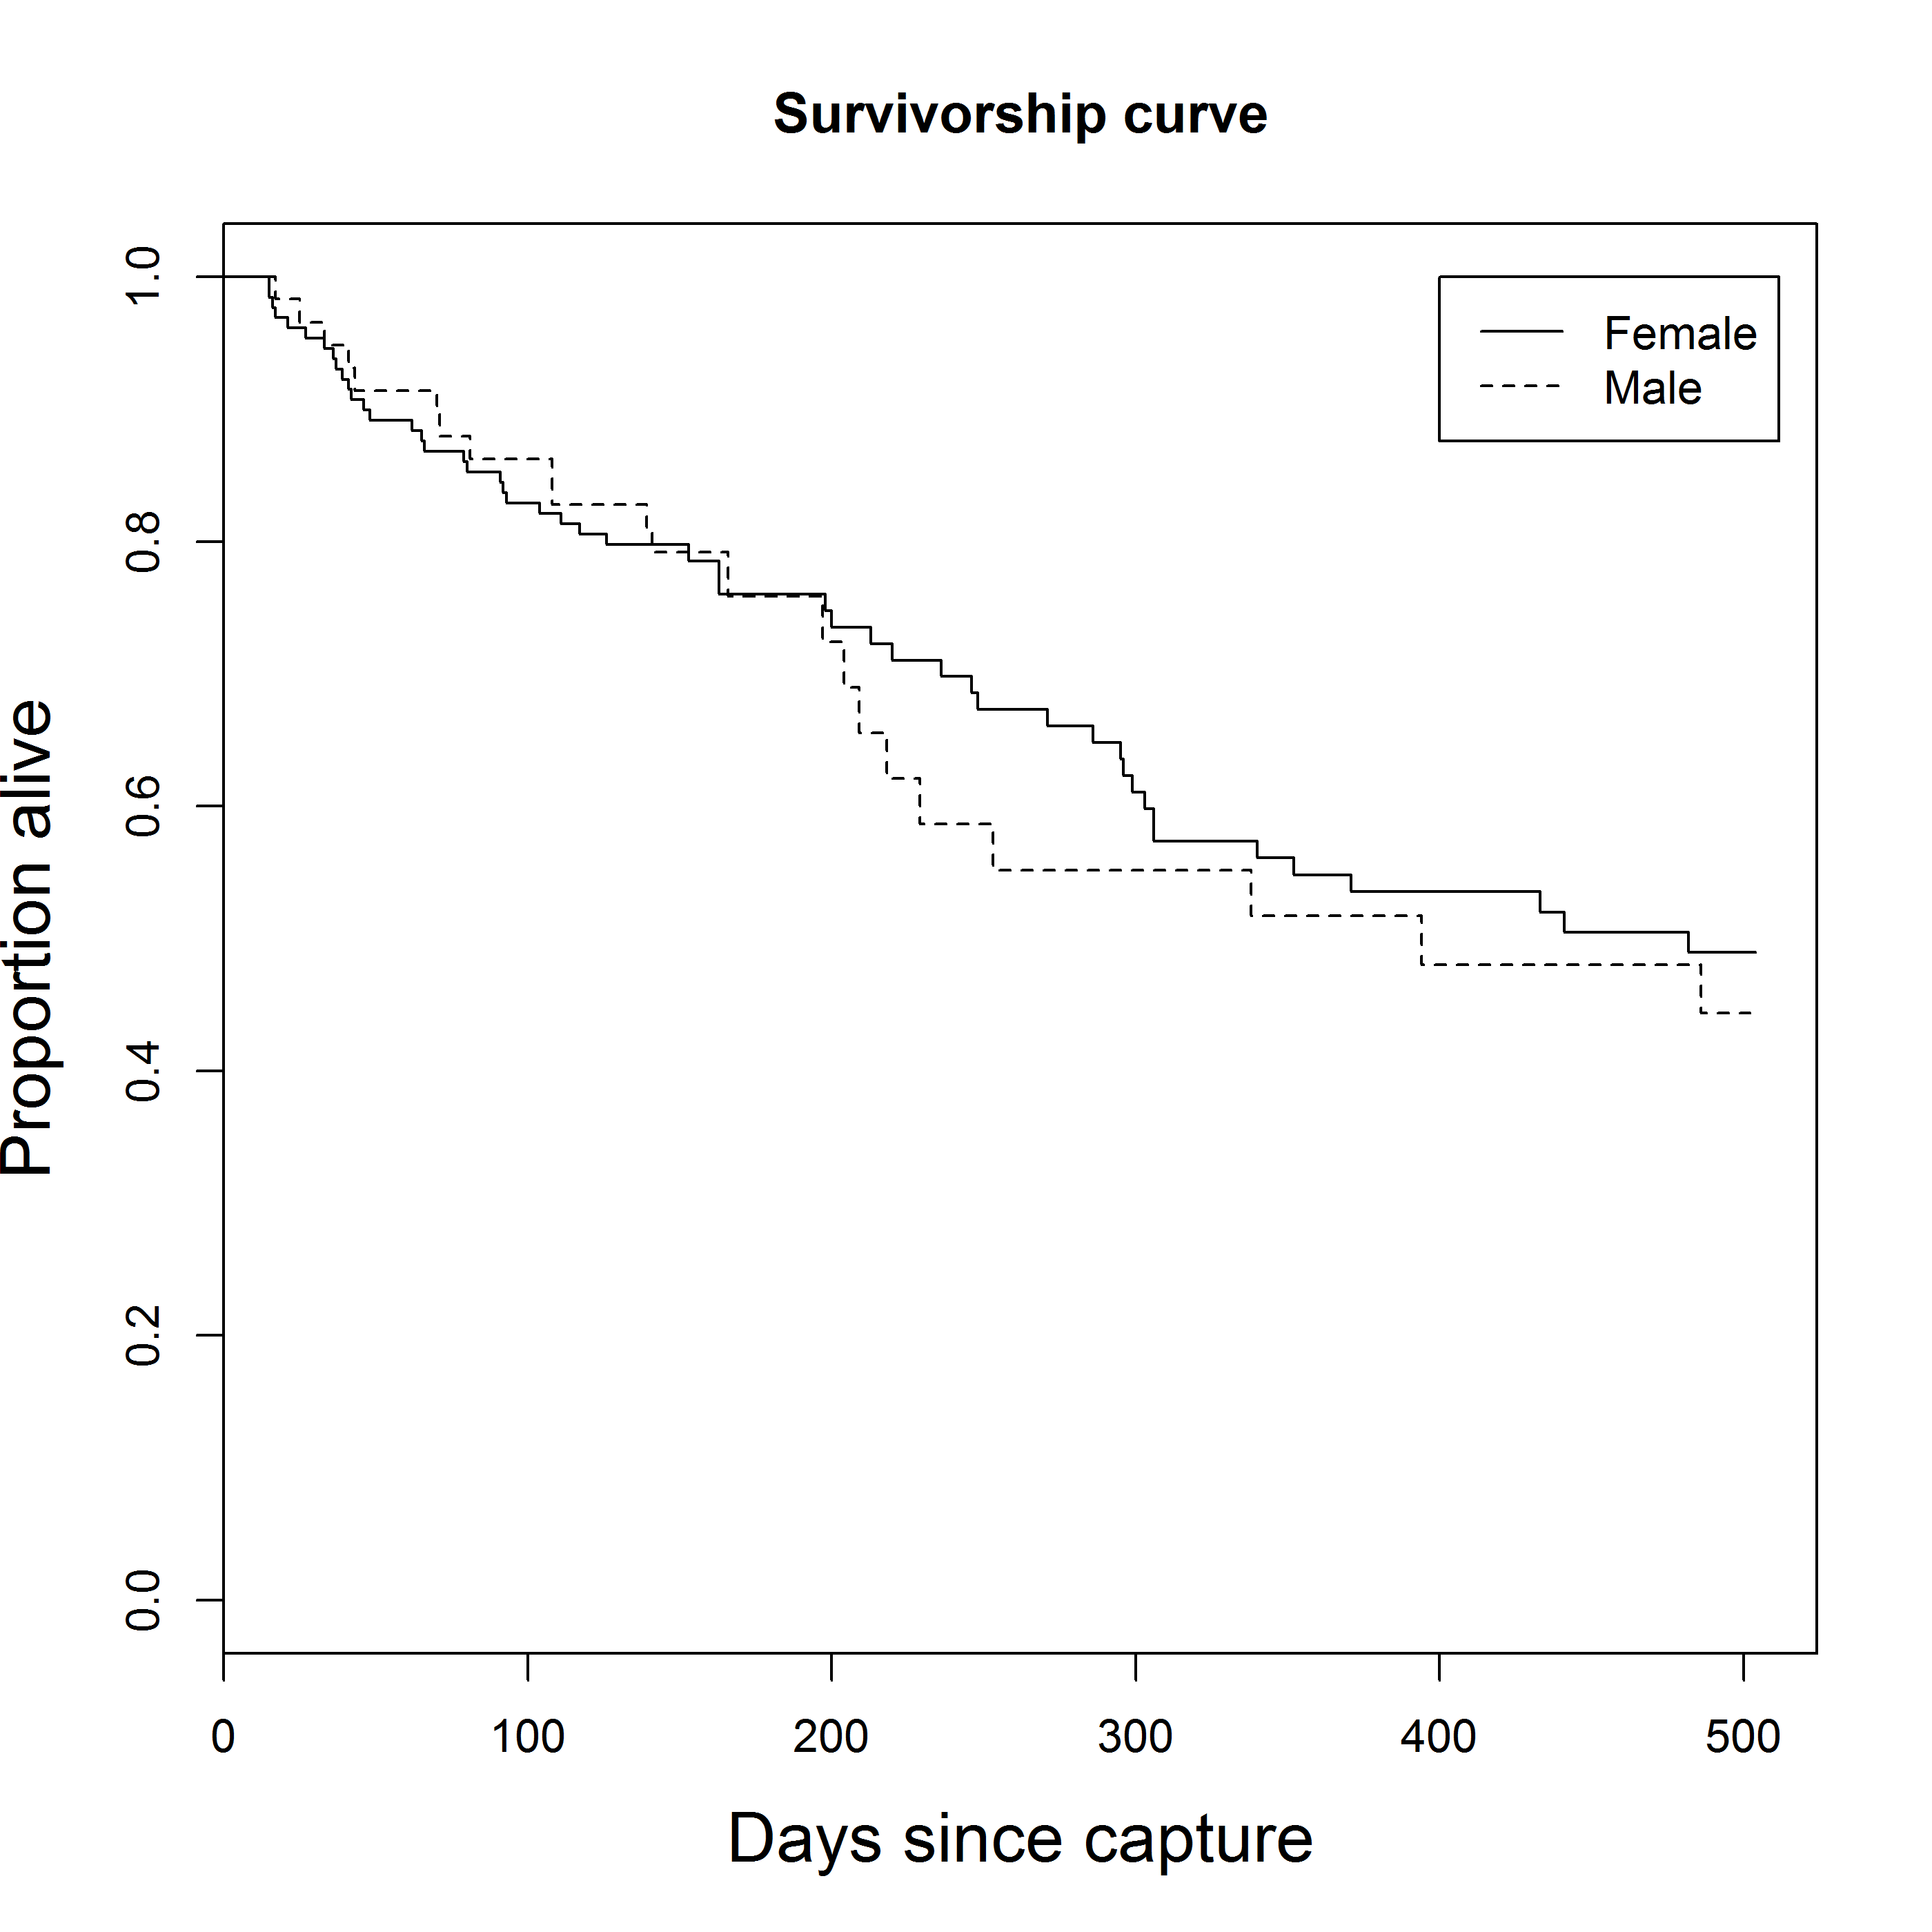
\includegraphics[width=0.70\textwidth]{deerSurv/deerSurvSex} \\
    \color{blue} 
    \url{
      https://youtu.be/Mgp46izlfeo
    }
  \end{center}
\end{frame}




\begin{frame}
  \frametitle{Kaplan-Meier}
  \large
  {\bf Critical Assumption}: \\
  Censoring must be independent of survival \\
 \begin{itemize}
   \item It's fine if transmitters fail randomly
   \item It's a problem if they fail because of mortality
 \end{itemize}
  \pause
  \vfill
%  {\bf }
%  \begin{itemize}
%    \item 
%  \end{itemize}
%  
%  \large
  {\bf Consequence of violating this assumption}: \\
  If an animal dies, but you mistakenly right censor it because you
  think its battery died, survival will be over-estimated.  
\end{frame}


\section{Age distributions}



\begin{frame}
  \frametitle{Age distribution data}
  {%\bf
    Standard practice}
  \begin{itemize}
    \item We have a pile of wings that can be aged \\
    \item We assume the age ratios tell us something about survival
  \end{itemize}
  \begin{center}
    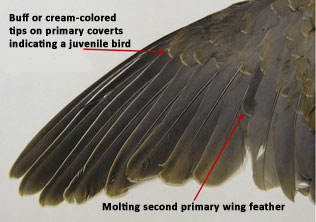
\includegraphics[width=0.6\textwidth]{figs/dove_wing}
  \end{center}
  \pause
%  Before considering this, let's image a better situation\dots
  {\centering \alert{\bf There are many problems with this} \par}
\end{frame}





\begin{frame}
  \frametitle{Alternative scenario}
%  \large
  Suppose a cohort of individuals is monitored over time, so that we
  can obtain information about survival.
  \Large
\[
  n_{i+1,t+1} = n_{i,t}S_{i,t}
\]
\pause
\[
  S_{i,t} = \frac{n_{i+1,t+1}}{n_{i,t}}
\]
% \large
\normalsize
\pause
\vfill
\centering %\bf
  All is well. This is a valid approach based on the
  binomial model. \\
\end{frame}



\begin{frame}
  \frametitle{Age distributions}
  \large
  The problem is that this\dots
  \Large
\[
  S_{i,t} = \frac{n_{i+1,t+1}}{n_{i,t}}
\]
  \pause
  \large
  \dots is not the same as data from ``standing age distribution''
  \Large
\[
  S_{i,t} = \frac{n_{i+1,t}}{n_{i,t}}
\]
\end{frame}




\begin{frame}
  \frametitle{Pitfall I}
  \large
  Standing age distribution data can't be used to estimate
    survival, unless\dots \\
  \begin{itemize}
    \item Population is at the stable age distribution
    \item $\lambda = 1$
  \end{itemize}
\end{frame}



\begin{frame}
  \frametitle{Pitfall II}
  \large
  {\bf Population reconstruction} refers to the calculation of the abundance
  and age distribution of a cohort at some initial time, usually based
  on ``ages at death''. \\
  \pause
  \vspace{0.5cm}
  This is only possible if we know the ages of death for \alert{\bf all}
  individuals in the cohort. \\
  \pause
  \vspace{0.5cm}
  Shouldn't use this type of ``reconstruction data'' as real data in a
  subsequent analysis.
\end{frame}




\begin{frame}
  \frametitle{Pitfall III}
  {\large %\bf
    The age data are biased \\}
  \large
  \begin{itemize}
    \normalsize
    \item Age data not representative of actual age distribution
    \item Hunting, trapping, and capture-recapture methods do not
      evenly sample the population
  \end{itemize}
\end{frame}





\begin{frame}
  \frametitle{Avoiding the pitfalls}
  \large
  %\bf
    When estimating survival, it is always good to\dots \\
  \begin{itemize}
    \normalsize
    \item Collect more than 1 year of data
    \item Follow multiple cohorts of individuals over long periods of time
    \item Estimate survival using telemetry or mark-recapture methods
  \end{itemize}
\end{frame}



\end{document}

% \begin{frame}
%   \frametitle{Assignment}
%   \LARGE
%   {\centering \bf Read Chapter 12 from Conroy and Carroll \par}
% \end{frame}




% \end{document}
